\chapter{Resultados}
\label{chap:result}

Este capítulo apresenta os principais resultados obtidos com o desenvolvimento do sistema, por meio de diagramas que ilustram as funcionalidades, a arquitetura e as interações entre os componentes da aplicação. Os diagramas foram elaborados com o objetivo de representar visualmente a estrutura e o funcionamento do sistema, facilitando a compreensão do seu comportamento e da sua modelagem. A seguir, são apresentados o diagrama de casos de uso, o diagrama de sequência e o diagrama de classes, cada um desempenhando um papel fundamental na documentação e análise do sistema.



\section{Diagrama de Casos de Uso}
\label{sec:casos}

O diagrama de casos de uso, apresentado na Figura \ref{fig:diagrama_uso}, representa as principais funcionalidades oferecidas pelo sistema e a forma como os atores interagem com ele. 

No sistema desenvolvido, existem dois atores principais: o \textbf{Desenvolvedor} e o \textbf{Usuário}. O Desenvolvedor tem permissão para \textit{Alterar Portfólio}, além de disponibilizar funcionalidades de visualização para o Usuário. Ambos os atores podem acessar os casos de uso de \textit{Visualizar perfil GitHub}, \textit{Visualizar perfil do LinkedIn} e \textit{Visualizar diploma}. 

Esses casos de uso demonstram as funcionalidades básicas voltadas à exibição de informações do portfólio do Desenvolvedor, com o objetivo de permitir que o Usuário visualize os conteúdos públicos disponibilizados.

\begin{figure}[h!]	
    \centering
    \caption{Diagrama de casos de uso}
    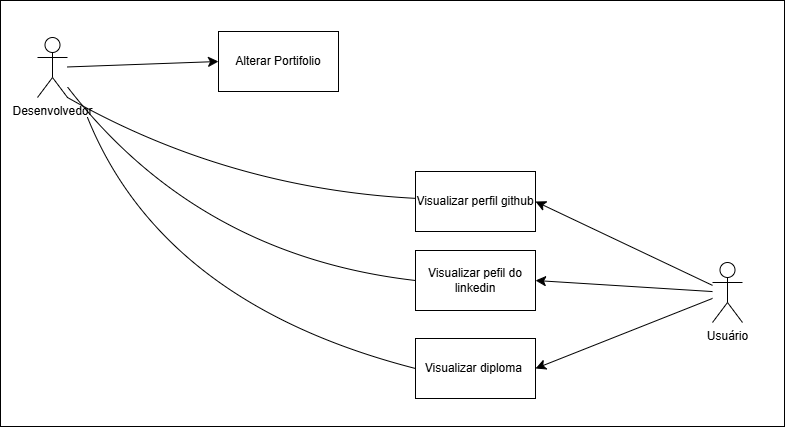
\includegraphics[width=0.8\textwidth]{Figures/diagrama_caso_uso.drawio.png}
    \caption*{Fonte: Autoria própria.}
    \label{fig:diagrama_uso}
\end{figure}

\clearpage
\section{Diagrama de Sequência}
\label{sec:sequencia}   

O diagrama de sequência, apresentado na Figura \ref{fig:diagrama_sequencia}, ilustra de forma detalhada o fluxo de interações entre os objetos do sistema ao longo do tempo para a realização de uma funcionalidade específica. Nele, é possível acompanhar a ordem cronológica das operações e a comunicação entre os componentes envolvidos, reforçando a dinâmica do comportamento do sistema.

Na sequência mostrada, o processo se inicia com a ação do \textbf{Usuário}, que, ao interagir com a interface (por exemplo, clicando em um elemento para visualizar um diploma ou acessar um link de rede social), desencadeia uma série de eventos. A \textbf{Interface de Usuário} registra esse evento e encaminha uma solicitação para o \textbf{Controlador} do sistema, que é responsável por processar a ação e gerenciar a lógica de negócio.

Após receber a solicitação, o Controlador realiza as seguintes etapas:
\begin{enumerate}
    \item Validação dos dados e verificação da integridade da requisição.
    \item Interação com a \textbf{Camada de Dados} para a recuperação das informações necessárias, como detalhes do diploma ou dados de perfis externos.
    \item Processamento dos dados recebidos e formatação da resposta para apresentação.
\end{enumerate}

Em seguida, o resultado desse processamento é devolvido ao usuário por meio da interface, seja na forma de uma exibição dinâmica (como a abertura de um modal com o diploma correspondente) ou do redirecionamento para uma página externa (como o perfil do LinkedIn ou GitHub).

Este diagrama evidencia a importância de uma comunicação clara e ordenada entre os componentes do sistema, assegurando que cada interação seja tratada de forma eficiente e que o fluxo de informações responda de maneira adequada às ações do usuário.

\begin{figure} [h!]	
    \centering
    \caption{Diagrama de sequencia}
    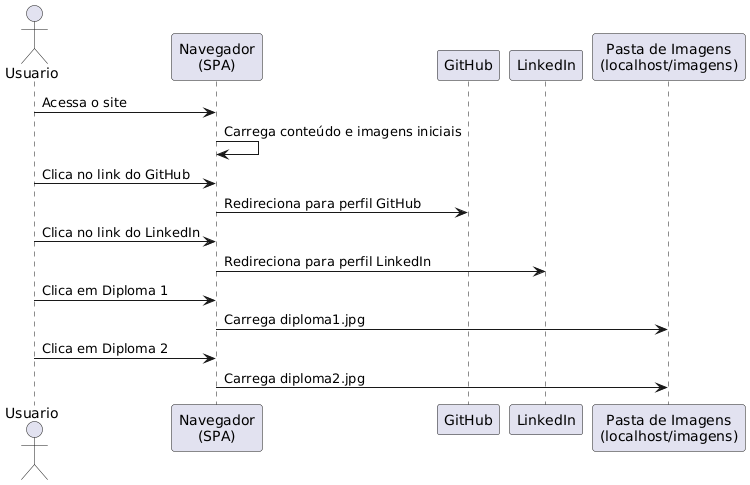
\includegraphics[width=0.8\textwidth]{Figures/diagrama_sequencia.png}
    \caption*{Fonte: Autoria própria.}
    \label{fig:diagrama_sequencia}
\end{figure}

\clearpage

\section{Diagrama de Classe}
\label{sec:classe}

O diagrama de classe, apresentado na Figura \ref{fig:diagrama_classe}, representa de forma estática a estrutura do sistema, evidenciando as classes que o compõem, seus atributos e os relacionamentos existentes entre elas. Essa representação facilita a compreensão da organização dos dados e das responsabilidades de cada entidade dentro do sistema.

No diagrama, a classe central é a Usuario, que possui atributos como fotoPerfil (do tipo FotoPerfil), foto (do tipo Foto), nome (do tipo string), além dos atributos diplomaUm e diplomaDois (ambos do tipo Diploma).

A classe Usuario está associada à classe Curriculo, indicando que um usuário pode possuir um currículo. A classe Curriculo contém atributos como usuario (do tipo Usuario), fotoUm e fotoDois (do tipo Foto), além de fotoGit e fotoLinkedin (ambos do tipo image).

Além disso, a classe Curriculo relaciona-se com a classe Projeto, permitindo que um currículo contenha múltiplos projetos. A classe Projeto possui atributos como curriculo (do tipo Curriculo) e mostrar\_projeto (também associado ao Curriculo).

Existem também classes auxiliares, como Diploma e FotoPerfil. A classe Diploma possui um atributo diploma (do tipo image), assim como a classe FotoPerfil que contém um atributo similar. Ambas são referenciadas pela classe Usuario, conforme indicado pelas linhas de associação no diagrama, sugerindo que um usuário possui ou utiliza instâncias dessas classes.

\begin{figure}[h!]
\centering
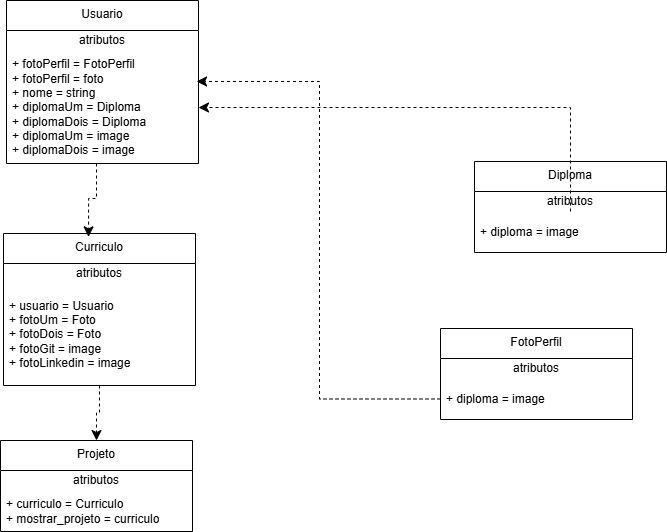
\includegraphics[width=0.8\textwidth]{Figures/diagrama_classe.drawio.png}
\caption{Diagrama de Classe do Sistema}
\caption*{Fonte: Autoria própria.}
\label{fig:diagrama_classe}
\end{figure}